\documentclass[11pt]{article}
\usepackage[margin=1.15in]{geometry}
\usepackage{amsmath,amssymb,amsthm}
\usepackage{booktabs}
\usepackage{graphicx}
\usepackage{microtype}
\usepackage[authoryear,round]{natbib}
\usepackage[colorlinks=true,linkcolor=black,citecolor=black,urlcolor=black]{hyperref}
\usepackage{setspace}
\onehalfspacing

\newtheorem{proposition}{Proposition}
\theoremstyle{definition}
\newtheorem{definition}{Definition}
\newcommand{\E}{\mathbb{E}}
\renewcommand{\Pr}{\mathbb{P}}

\title{Privileged Teachers\\[4pt]
\large What an Oracle Label Teaches a Selector Under Partial Observation}
\author{Flyxion\\Independent Researcher}
\date{October 2026}

\begin{document}
\maketitle

\begin{abstract}
\noindent
Training a decision module against an oracle that sees the true scene is a standard way to obtain labels when the deployed agent sees only a partial observation. The labels are correct for the oracle. They are not, in general, the labels that identify the best decision for an agent that cannot see what the oracle sees. This essay states the gap precisely. A classifier trained on oracle labels with cross-entropy learns the probability that an option is the oracle's choice, which ranks options differently from their expected value whenever payoffs are unequal. A regression head trained on the oracle's best-in-group outcome learns the expected maximum of a group, which exceeds the expected value of the item that will actually be executed by an amount that grows with the within-group spread and the group size and shrinks with the resolution of the within-group chooser. Both effects are computed in closed form for a Gaussian model and illustrated by simulation. A recent active-mapping system that trains its mode selector on ground-truth coverage gains is used as the worked example, because its appendix specifies the targets exactly. The conclusions concern what the targets estimate, not whether the system performs well, which its benchmarks address separately.
\end{abstract}

\section{A teacher that sees more than the student}

A standard device for training a policy from partial observations is to build a teacher that sees more: the true map, the true terrain, the true state. The teacher's actions are then used as labels or targets for a student that receives only what a deployed agent would receive. The device has produced strong systems, including legged locomotion trained against a teacher with privileged terrain information \citep{lee2020}, and it has a well-studied failure: the student can be unable to reproduce the teacher because the teacher's choice depends on information the student lacks, a situation called the imitation gap \citep{weihs2021,warrington2021}. Interactive imitation methods that query the expert on states the student visits address a related mismatch between the data distribution and the deployment distribution \citep{ross2011}.

The present essay is concerned with a different and more elementary question: what a given oracle target is an estimate of. The question is not whether the student can match the teacher. It is whether matching the teacher's statistics is what the deployed decision requires. Because the answer depends on the exact form of the target, the discussion uses a concrete system whose appendix specifies the targets. The system \citep{li2026} generates several exploration anchors with a conditional flow-matching model, plans a path to each, clusters the paths into modes, and selects a mode and then a path with a learned selector. In training, candidate paths are generated and scored on the ground-truth obstacle map, and the selector is supervised with oracle labels. The relevant specifications are, in the extended appendix, (i) a cross-entropy loss on an \emph{oracle positive mode}, the mode that contains the optimal path; (ii) a listwise ranking loss within the mode on the oracle-best path; and (iii) a squared-error loss for a mode gain head whose target is the \emph{maximum} actual coverage gain over the paths in the mode. The deployed score is a weighted sum of the heads and the mode with the highest score is chosen.

Each of these is a reasonable-looking choice. Each also estimates something specific, and the specific quantity is not the one that a rational agent with only the observation $z$ should maximize.

\section{Label frequency is not value}
\label{sec:label}

Let $S$ denote the full scene, $z$ the observation available to the agent, and $g(a,S)$ the realized gain of action $a$ in scene $S$. The oracle chooses $a^\ast(S)=\arg\max_a g(a,S)$. The agent chooses $a$ knowing only $z$, and its expected gain is $\E[g(a,S)\mid z]$.

\begin{proposition}
A classifier trained with cross-entropy on the oracle's choice $a^\ast(S)$, given $z$, converges to $p(a\mid z)=\Pr(a^\ast(S)=a\mid z)$. The decision that maximizes expected gain is $a^{B}(z)=\arg\max_a\E[g(a,S)\mid z]$. The two coincide when the payoff is the same whenever the oracle's choice is made, $g(a,S)=c\,\mathbf 1\{a=a^\ast(S)\}$. In general $\arg\max_a p(a\mid z)\neq a^B(z)$.
\end{proposition}

\begin{proof}
The first statement is the standard calibration property of the cross-entropy minimizer. If the payoff is $c\,\mathbf 1\{a=a^\ast(S)\}$ then $\E[g(a,S)\mid z]=c\,p(a\mid z)$ and the two rankings agree. For the general case, take two actions with $g(1,S)=G$ on an event of probability $q$ and $0$ otherwise, and $g(2,S)=\gamma$ with $0<\gamma<G$ always. The oracle chooses action~1 exactly when the event occurs, so $p(1\mid z)=q$, while $\E[g(1)]=qG$ and $\E[g(2)]=\gamma$. The label rule chooses action~1 iff $q>1/2$ and the value rule iff $q>\gamma/G$, and the two differ for $q$ between $\gamma/G$ and $1/2$ whenever $\gamma/G<1/2$.
\end{proof}

With $G=10$ and $\gamma=3$ the value rule chooses the risky option for $q>0.3$ and the label rule for $q>0.5$. At $q=0.4$ the label rule takes the certain gain of $3$ and forgoes an expected $4$. Table~\ref{tab:two} lists the cases. The two rules agree at the extremes and disagree in the intermediate range where the choice is hard, which is the range where a learned selector is most needed.

\begin{table}[h]
\centering
\caption{Two options. East pays $G=10$ with probability $q$ and $0$ otherwise; west pays $\gamma=3$ for certain. The oracle chooses east exactly when it pays.}
\label{tab:two}
\begin{tabular}{rcccc}
\toprule
$q$ & expected gain, east & expected gain, west & label rule & value rule \\
\midrule
0.2 & 2 & 3 & west & west \\
0.3 & 3 & 3 & west & tie \\
0.4 & 4 & 3 & west & east \\
0.5 & 5 & 3 & west & east \\
0.7 & 7 & 3 & east & east \\
\bottomrule
\end{tabular}
\end{table}

The point is not specific to this toy. Whenever outcomes differ in size, the frequency with which an option is best and the amount it yields on average are different functionals of the same conditional distribution. A system whose generator proposes alternatives and whose selector ranks them by expected value is insulated from this, since the generator's matching of oracle frequencies then only determines what is proposed. The cross-entropy label on the oracle's mode is where the frequency enters the decision. The system's total score also contains regression heads, so what the deployed ranking inherits depends on the weights $\lambda$ of the training objective and on the learned $w$ of the score, neither of which is reported as an ablation in the text examined. The question is therefore not settled by the argument above, only localized by it.

\section{A maximum is not an expectation of what is executed}
\label{sec:max}

The mode gain head is trained against
\begin{equation}
G_m^{\mathrm{GT}}=\max_{\tau\in\mathcal M_m}\Delta\mathrm{Cov}(\tau),
\label{eq:target}
\end{equation}
where $\Delta\mathrm{Cov}(\tau)$ is the actual coverage gain from executing path $\tau$. The appendix states the reason for the maximum: mode-level selection is meant to ask whether a mode contains a high-quality path, the upper bound of its potential. That is a stated design choice and it is consistent with a hierarchy in which a second stage picks the best path within the chosen mode.

What the head learns, under squared error, is $\E[\max_{\tau\in\mathcal M_m}\Delta\mathrm{Cov}(\tau)\mid z,m]$, the expected best-in-mode gain over scenes consistent with the observation. What the system delivers once it has chosen the mode is the gain of the single path the local reranker picks. The reranker is itself trained on the oracle-best path but, at test time, ranks from the observation. The difference between the two quantities is a value-of-information term. A mode whose paths all have similar gains has little of it. A mode with many paths whose gains differ in ways the observation does not reveal has a lot, and the maximum over scenes pays for exactly that unseen variation.

A Gaussian model makes the size explicit.

\begin{proposition}
Suppose mode $m$ has $n$ paths with gains $\mu+\sigma\epsilon_j$, with $\epsilon_j$ independent standard normal given $z$. Let the reranker choose the path maximizing a signal $s_j=\rho\,\epsilon_j+\sqrt{1-\rho^2}\,\eta_j$ with $\eta_j$ independent standard normal noise, $0\le\rho\le1$. Then the expected best-in-mode gain is $\mu+\sigma c_n$ and the expected executed gain is $\mu+\sigma\rho\, c_n$, where $c_n=\E\max_{j\le n}\epsilon_j$. The overstatement is
\begin{equation}
\E[\max]-\E[\text{executed}]=\sigma(1-\rho)\,c_n .
\end{equation}
\end{proposition}

\begin{proof}
The first expression is the mean of the maximum. For the second, the selected index maximizes $s_j$, so the executed gain is $\mu+\sigma\epsilon_{j^\ast}$. Since $\epsilon_{j^\ast}\mid s_{j^\ast}$ has mean $\rho s_{j^\ast}$ and the signals are exchangeable with unit variance, $\E[\epsilon_{j^\ast}]=\rho\,\E[\max_j s_j]=\rho c_n$.
\end{proof}

The coefficient $c_n$ increases slowly with group size: by Monte Carlo (200{,}000 draws) $c_2=0.57$, $c_4=1.03$, $c_8=1.42$, $c_{16}=1.77$. With $\rho=0.4$, a mode of 16 paths whose gains have standard deviation $\sigma$ is overstated by $1.06\,\sigma$, against $0.34\,\sigma$ for a mode of two. Two modes with the same executed value but different spread and size therefore receive different scores, and the score favors the more dispersed and more populous one.

The size of the effect depends on $\rho$, which the paper does not report: how well the local reranker identifies the in-mode best path. If the reranker is nearly perfect, the maximum is an excellent proxy for the executed gain and the design is justified. If it is poor, the target rewards spread. The relevant evidence is the gain head's prediction compared with the realized gain of the path actually executed, binned by mode size and by within-mode spread. The benchmark tables do not contain it.

\section{How much it could matter}

A simulation puts numbers on the two effects together. Each trial draws $K=4$ modes with means $\mu_m\sim\mathcal N(0,1)$, spreads $\sigma_m\sim U(0.2,2)$, and sizes $n_m\sim U\{2,\dots,16\}$. For $4000$ scene draws, path gains are $\mu_m+\sigma_m\epsilon$ with the reranker model above. Three scoring rules choose a mode: the true expected executed gain (the value rule, which defines regret), the expected best-in-mode gain as in \eqref{eq:target}, and the probability that the mode contains the best path in the scene as in the oracle positive-mode label. Regret is the executed value of the best mode minus that of the chosen one, in the units of $\mu$.

\begin{table}[h]
\centering
\caption{Mean regret and disagreement with the value rule, by reranker resolution $\rho$ (400 trials each, $K=4$ modes). Standard errors of the regrets are about $0.02$ at $\rho=0$, $0.009$ at $0.4$, $0.004$ at $0.7$ and $0.0006$ at $0.9$.}
\label{tab:regret}
\small
\begin{tabular}{rcccc}
\toprule
$\rho$ & \multicolumn{2}{c}{mean regret} & \multicolumn{2}{c}{different mode from value rule} \\
 & best-in-mode & oracle label & best-in-mode & oracle label \\
\midrule
0.0 & 0.265 & 0.265 & 40\% & 40\% \\
0.4 & 0.067 & 0.071 & 19\% & 20\% \\
0.7 & 0.019 & 0.023 & 10\% & 11\% \\
0.9 & 0.002 & 0.002 & 3\% & 3\% \\
\bottomrule
\end{tabular}
\end{table}

The regrets are not large in absolute terms, since the toy modes' means have unit spread, and they vanish as $\rho\to1$. The disagreement rate is the more informative column: when the chooser cannot resolve paths within a mode, the two oracle-derived scores pick a different mode from the value rule in two of five decisions, and even at $\rho=0.4$ in about one of five. The two oracle-derived rules behave alike in this model because both reward the same property, the chance of containing a very good path. Combining them in one score does not cancel the effect.

\begin{figure}[h]
\centering
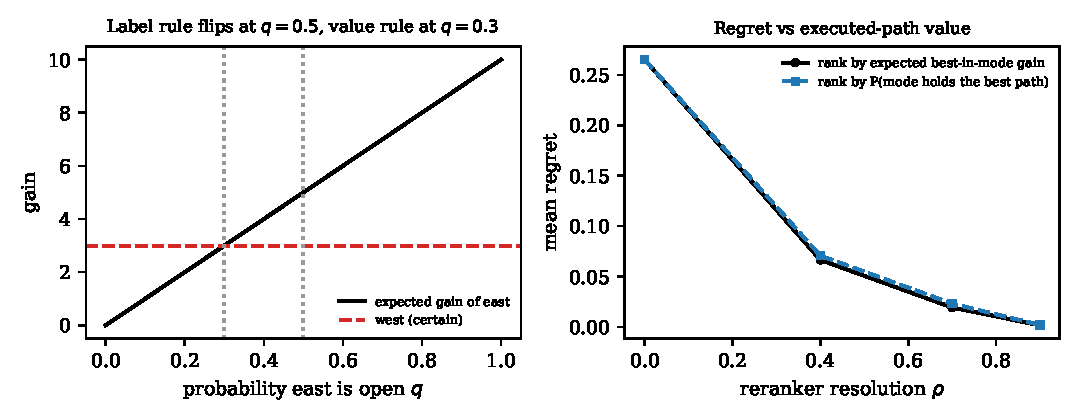
\includegraphics[width=\textwidth]{fig_teach.pdf}
\caption{Left: the expected-gain and certain-gain lines of Table~\ref{tab:two}; the label rule changes option at $q=0.5$ and the value rule at $q=0.3$. Right: mean regret against the value rule as reranker resolution $\rho$ increases (Table~\ref{tab:regret}).}
\label{fig:teach}
\end{figure}

The simulation is a stylized model and not an estimate for the system in question. Its role is to show that the direction of the effect is robust to the specifics, and that the magnitude is governed by two quantities, within-mode spread and reranker resolution, that can be measured.

\section{What the reported ablation separates}

The component analysis in the main text reports a progressive build-up under a cross-dataset setting: adding multimodal anchor generation raises completion from 61.81\% to 66.21\%, mode clustering to 67.60\%, and hierarchical selection to 68.45\%, with the distance metric moving from 9.36 to 9.11 cm in the last step. The last step bundles the mode-level scorer and the local reranker together with all their loss terms. It therefore cannot indicate whether the cross-entropy label, the maximum-gain target, the mean-gain target, or the risk and uncertainty heads contributed, or whether any of them cost performance that others recovered. The results are consistent with the selector helping and with the selector helping despite the bias described here. They do not distinguish between them, and no statement about the bias is a statement that the selector is harmful.

The experiments that would separate the cases are inexpensive relative to the system. First, train the mode scorer with the mean over paths in the mode, or the realized gain of the path the reranker picks, in place of the maximum in \eqref{eq:target}, and compare. Second, remove the cross-entropy mode label and keep the regression heads, and the reverse. Third, report the calibration of the gain head against executed gain by mode size and spread. Fourth, train the selector on states visited by the student's own policy, relabeled by the oracle, to address the distribution mismatch that interactive imitation targets \citep{ross2011}. The passages examined do not state which state distribution the selector is trained on, and the answer affects whether the label statistics in Section~\ref{sec:label} are even the ones met at deployment.

\section{What follows}

An oracle target estimates the oracle's behavior, aggregated over everything the student cannot see. Three habits keep the aggregation honest.

\paragraph{Ask what the loss converges to.} Cross-entropy on an oracle choice converges to a choice frequency. Squared error on an oracle statistic converges to that statistic's conditional mean. Naming the limit is usually enough to see whether it is the quantity that the downstream decision rule needs.

\paragraph{Match the target to the executed action.} If a stage will execute one path, the value to be predicted is the value of that path under the policy that will pick it, not the best path an informed observer could have chosen. The maximum is a legitimate target for a different question, namely how much could be gained with more information.

\paragraph{Report the resolution of each stage.} The costs of the maximum-style targets scale with how poorly the later stage resolves the choices, and a hierarchy of stages needs its inter-stage resolution reported, since each stage's score is partly an estimate of what the next stage can do.

A teacher with privileged information is a useful instrument. What it knows is not the student's to know, and the targets derived from it carry that difference into the student's decisions unless the loss is chosen to remove it.

\begin{thebibliography}{9}
\bibitem[Lee et al.(2020)]{lee2020} Lee, J., Hwangbo, J., Wellhausen, L., Koltun, V., Hutter, M. (2020). Learning quadrupedal locomotion over challenging terrain. \emph{Science Robotics} 5(47), eabc5986.
\bibitem[Li et al.(2026)]{li2026} Li, Y., Wu, A., Zhang, Z., Han, Z., Zhang, S., Han, Y. (2026). All roads lead to Rome: flow-driven multi-anchor exploration for open-environment active 3D mapping. arXiv:2609.36889.
\bibitem[Ross et al.(2011)]{ross2011} Ross, S., Gordon, G., Bagnell, J.~A. (2011). A reduction of imitation learning and structured prediction to no-regret online learning. \emph{Proceedings of the 14th International Conference on Artificial Intelligence and Statistics (AISTATS)}, PMLR 15, 627--635.
\bibitem[Warrington et al.(2021)]{warrington2021} Warrington, A., Lavington, J.~W., Scibior, A., Schmidt, M., Wood, F. (2021). Robust asymmetric learning in POMDPs. \emph{Proceedings of the 38th International Conference on Machine Learning}, PMLR 139.
\bibitem[Weihs et al.(2021)]{weihs2021} Weihs, L., Jain, U., Liu, I.-J., Salvador, J., Lazebnik, S., Kembhavi, A., Schwing, A. (2021). Bridging the imitation gap by adaptive insubordination. \emph{Advances in Neural Information Processing Systems} 34.
\end{thebibliography}

\end{document}
